\chapter{Evaluation}

%EL schemas enable consistent, structured, and interpretable inferences about novel text, by matching pieces of the text to pieces of the schema, replacing schema variables with entities from the story, and treating other formulas in the schema that use those newly-filled variables as inferences. Here, we describe an assessment of the generality and relevance of the schema formulas learned by NESL.
%In addition to inferences, we would like to evaluate whether the schemas we obtain are both \textit{topically cohesive}, i.e., focused descriptions of one kind of situation; and \textit{interesting}, i.e., capable of generating useful and novel inferences about situations, rather than obvious or redundant ones.
This chapter describes experiments performed to assess the quality of schemas learned by NESL, and of inferences generated by learned schemas on unseen stories.
One way of evaluating acquired script-like knowledge is the \textit{narrative cloze} task, introduced by \citet{chambers2008unsupervised}, in which one event in a sequence is masked, and acquired knowledge is used to predict its identity given the rest of the sequence.
The narrative cloze task has been widely adopted as a standard evaluation for script-like knowledge acquisition \citep{jans-etal-2012-skip,rudinger-etal-2015-learning,pichotta2016learning,lee-goldwasser-2019-multi}.
However, \citet{rudinger-etal-2015-learning} note that the format of the narrative cloze task essentially mirrors that of a language model objective function, in which a missing token is predicted given a preceding sequence (in the autoregressive objective) or surrounding sequences (in the masked objective).
They argue that either discriminative language models are sufficient for the acquisition of script knowledge, or the narrative cloze task is insufficient for its evaluation.
\citet{chambers-2017-behind} defends the event cloze task by pointing out that many of its implementations, in automatically generating their evaluation sets, tested for non-representative distributions of events favoring high-frequency ones.
They argue for manual construction of narrative cloze tests by human annotators, with an emphasis on the inclusion of \textit{core} script events.

While NESL uses a generative language model to produce stories as an initial source for schema knowledge, the knowledge encoded in the final schemas is not drawn from the same distribution as the one producing the stories; stories often elide basic, but important, information about goals, preconditions, postconditions, and general semantic role types, which we introduce via protoschema identification. Furthermore, generative models of stories may call for the introduction of surprising events or facts in accordance with larger-scale \textit{narrative} schemas---this to the semantic detriment of the more basic, unsurprising schemas we'd like to extract from stories. Because of these factors contributing to the potentially highly disjoint event spaces of individual stories and learned schemas, we believe that a narrative cloze task is insufficient to test the quality and utility of the inferences generated by NESL-learned schemas, and employ human evaluation of learned schemas and their inferences. The remainder of this chapter describes the evaluation of schema steps and goals given the schema topic (Section~\ref{sec:schema_eval}), and the evaluation of concrete inferences, drawn using learned schemas, about unseen stories (Section~\ref{sec:inf_eval}).

\section{Schema Evaluation}
\label{sec:schema_eval}
Our first study evaluated the quality of individual schema formulas learned by NESL. We presented learned schema formulas from the \texttt{:Steps} and \texttt{:Goals} sections to human annotators and asked them to rate the quality of the formula, given the schema topic, on a 1-5 Likert scale. The prompt given to the evaluators was the following:
\begin{displayquote}
\textit{The statement above is a reasonably clear, entirely plausible general claim and seems neither too specific nor too general or vague to be useful.}
\end{displayquote}
This prompt is due to \citet{knext-eval}, who used it to elicit evaluations of quality of automatically acquired knowledge formulas from the \texttt{KNEXT} acquisition system. It incorporates three key dimensions into one quality rating: \textbf{clarity} of the representation, and \textbf{plausibility} and \textbf{generality} of the claim.

Prior work on human evaluation of automatically acquired script-like knowledge has used comparable study design. We compare our results to \citet{pichotta2016learning}, whose inferred event tuples were rated on a Likert scale, with values ranging from \textit{Very Unlikely} to \textit{Very Likely}, by human evaluators. While the semantics of the prompt are more ambiguous than our \texttt{KNEXT}-derived prompt, the normalized results are more or less comparable. \citet{weber_causal_scripts} evaluate acquired knowledge using two metrics, one of which is the \textit{event chain completion} metric, in which human evaluators rate the likelihood of a predicted event given a chain of preceding events. The comparison of this metric to ours is arguably the least direct, as we evaluate the likelihood of an event predicated on the truth of the schema's \textit{topic}; however, under the assumption that the given events in the event chain completion metric sufficiently characterize an implicit schema topic to the human evaluator, a comparison is possible. \citet{goal-oriented-scripts} ask human evaluators to \textit{edit} learned scripts by either re-ordering their steps or deleting irrelevant steps. This leads to an approximation of schema relevance defined by the ratio of edited script length to original script length, i.e. how many of the learned events were judged to be irrelevant. \citet{starsem-scripts} manually evaluate their own script events for topical relevance, among other things.

\begin{figure}
    \centering
    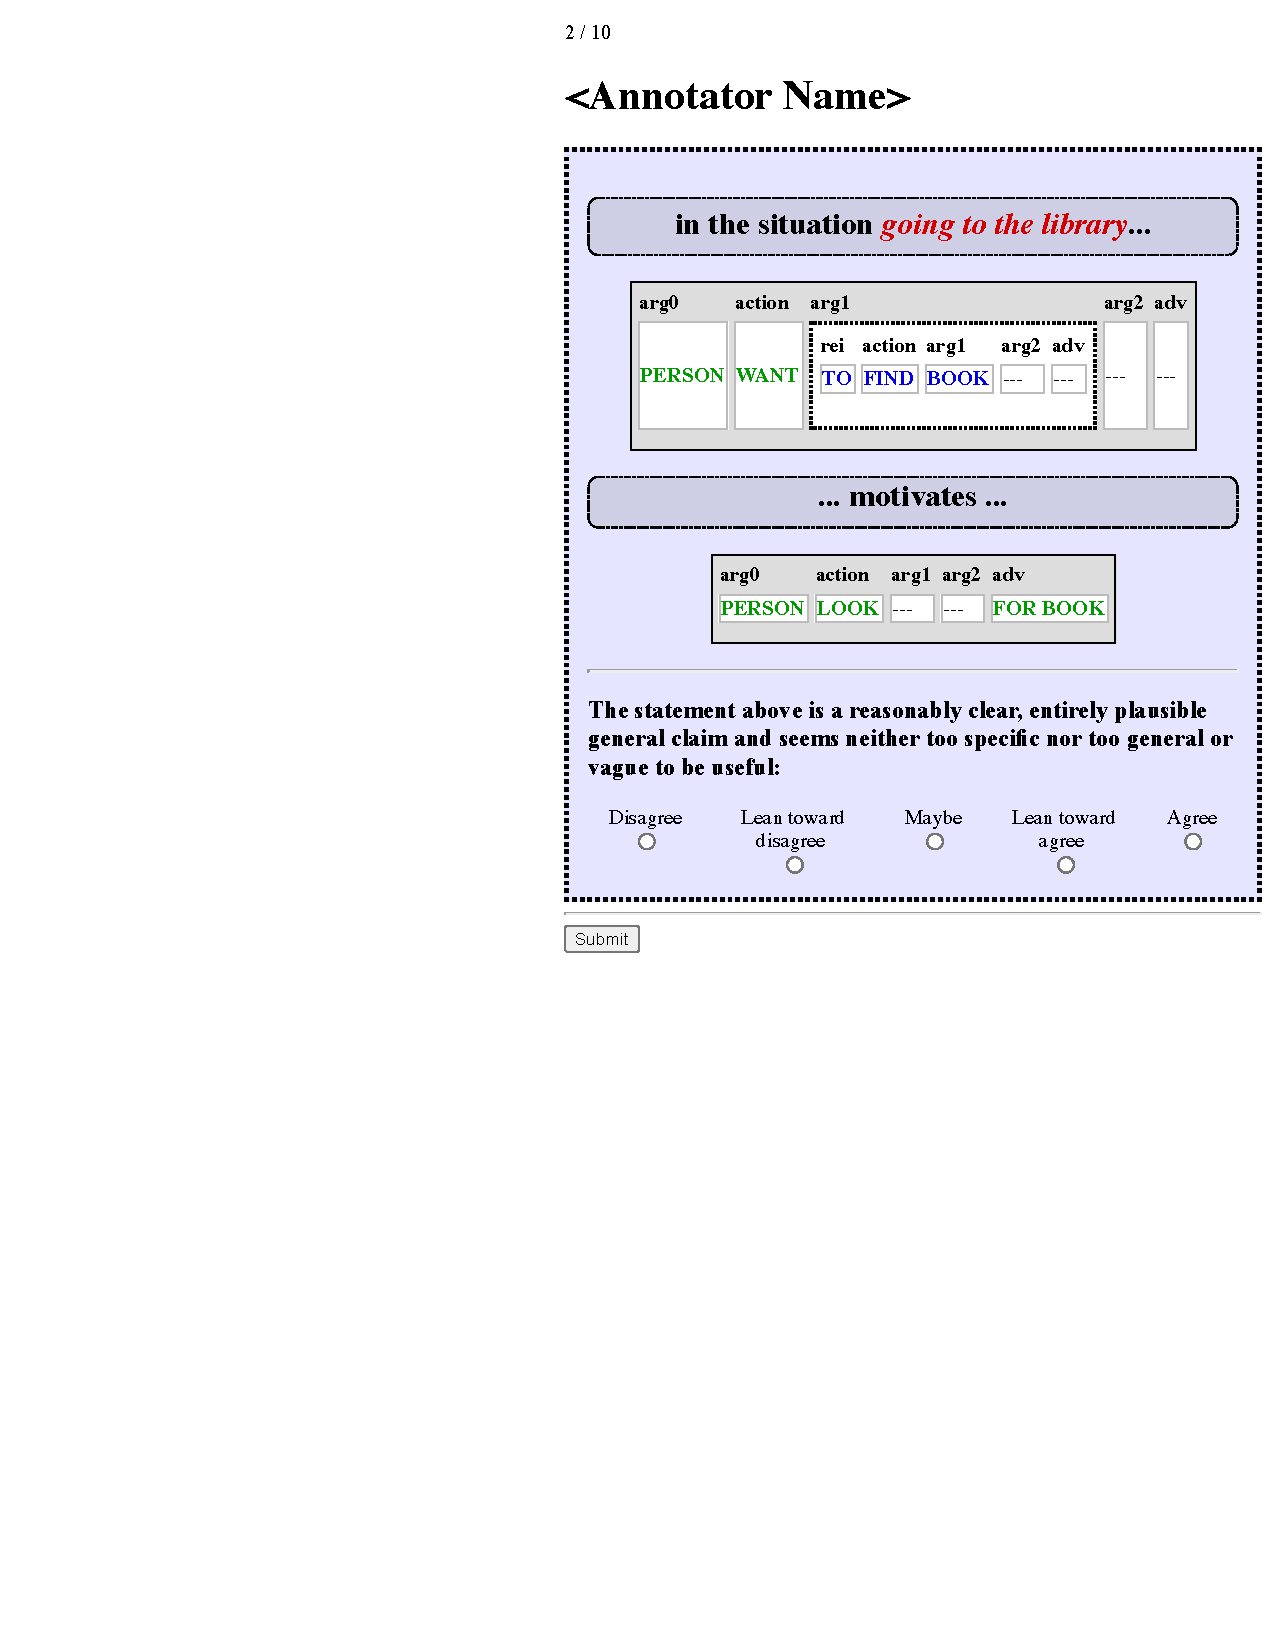
\includegraphics[width=0.5\textwidth]{CH4_learning/evaleg4.pdf}
    \caption{An example of a form presented to a schema quality evaluator for a \textit{goal} formula.}
    \label{fig:goal_eval_eg}
\end{figure}

For each step and goal formula in each learned schema, we first constructed a \textit{tabular representation} (tabrep), meant to render the EL formula in a human-readable way while still illustrating its formal predicate-argument structure. Two examples of tabreps can be seen in Figure~\ref{fig:goal_eval_eg}, which contains representations of the formulas \el{(?X (WANT.V (KA (FIND.V ?B))))} and \el{(?X ((ADV-A (FOR.P ?B)) LOOK.V))}, with context role type formulas \el{(?X PERSON.N)} and \el{(?B BOOK.N)}. Each tabrep has slots for \texttt{arg0}, the prefix argument; \texttt{action}, the verb predicate; \texttt{adv}, for single adverbial modifiers derived from monadic prepositional predicates; and \texttt{arg1} and \texttt{arg2}, for up to two postfix verb arguments. Arguments in tabreps can also recursively nest other tabreps, such as in the first (top) example in in Figure~\ref{fig:goal_eval_eg}; because tabreps represent actions or events, they must be reified to act as arguments, and thus the reifier (\texttt{TO}, a.k.a. \el{KA}, in the example) is represented in the \texttt{rei} slot of any nested tabrep. Leaf-level tabrep slot fillers are single words derived either from the lexical form of the verb or preposition predicate, or the first noun type predicate for the individual as found in the context formulas.

Left-to-right linearizations of nested tabreps are designed to be interpretable by untrained evaluators as crude English sentences. However, to demonstrate the end-to-end applicability of EL schemas to natural language inference, we also experimented with further refinement of tabreps into natural language using transformer-based language models. For each of 3,783 sentences derived from 913 stories generated by GPT-J 6B \footnote{20 stories were generated for each of 50 topics not used for the generation of schemas in the experiment. Empty stories and unparseable sentences were discarded, leaving 913 stories and 3,783 sentences.}, we parsed ELFs, formed tabreps, and linearized the tabreps into crude sentences. Like in the \texttt{ulf-gpt2} project detailed in Section~\ref{sec:ulf-gpt2}, we then created pairs of the form \begin{center}
\texttt{THIS BE EXAMPLE \textbf{<SEP>} This is an example. \textbf{<END>}}
\end{center}
for the crude and natural versions of each sentence and fine-tuned a \texttt{gpt2-large} model on the corresponding set of pairs. The crude sentence comes first due to the autoregressive nature of the language model. The resulting fine-tuned language model was used to create final, more fluent English verbalizations of the ELFs evaluated in the study. An example of a fluent sentence, computed from a tabrep by the language model, is shown in the evaluation form in Figure~\ref{fig:gpt_step_eval_eg}; its corresponding tabrep is shown in the form in Figure~\ref{fig:step_eval_eg}.

\begin{figure}
    \centering
    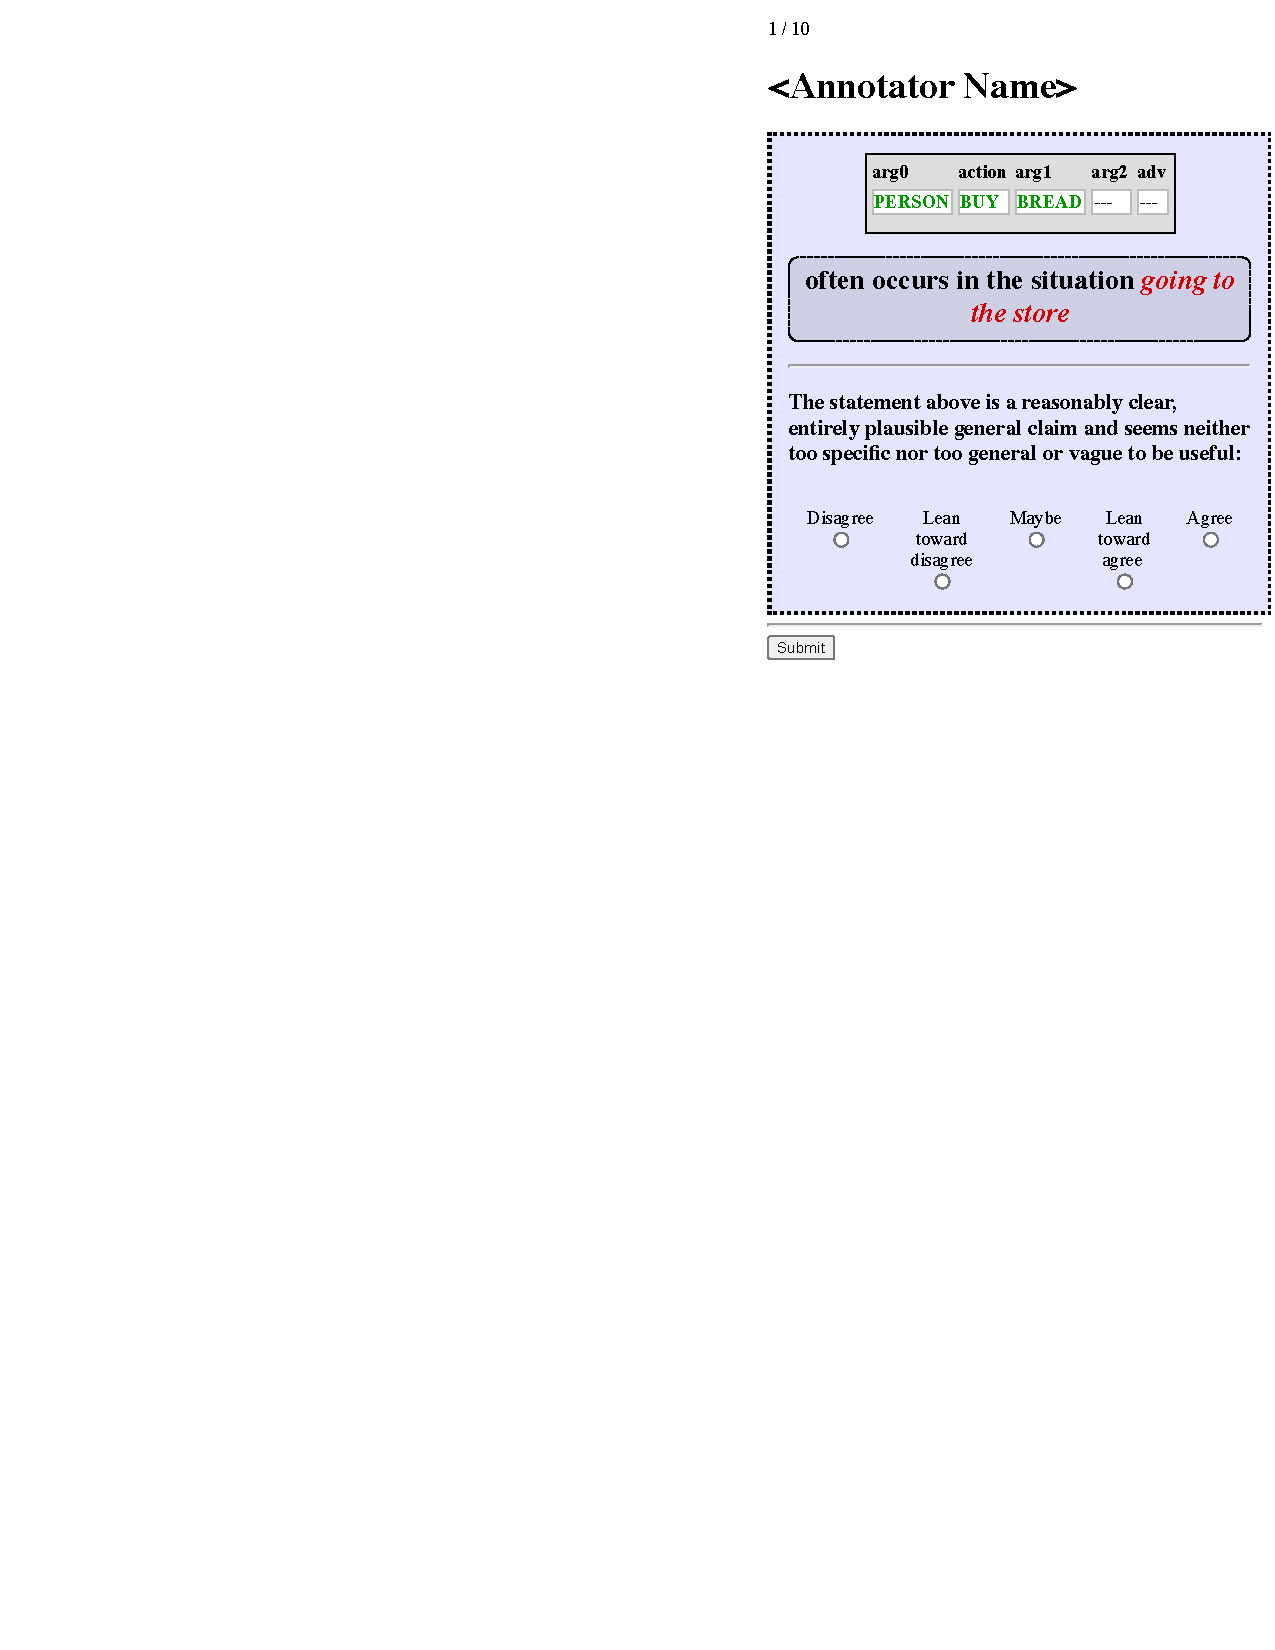
\includegraphics[width=0.5\textwidth]{CH4_learning/evaleg3.pdf}
    \caption{An example of a form presented to a schema quality evaluator for a \textit{step} formula.}
    \label{fig:step_eval_eg}
\end{figure}

\begin{figure}
    \centering
    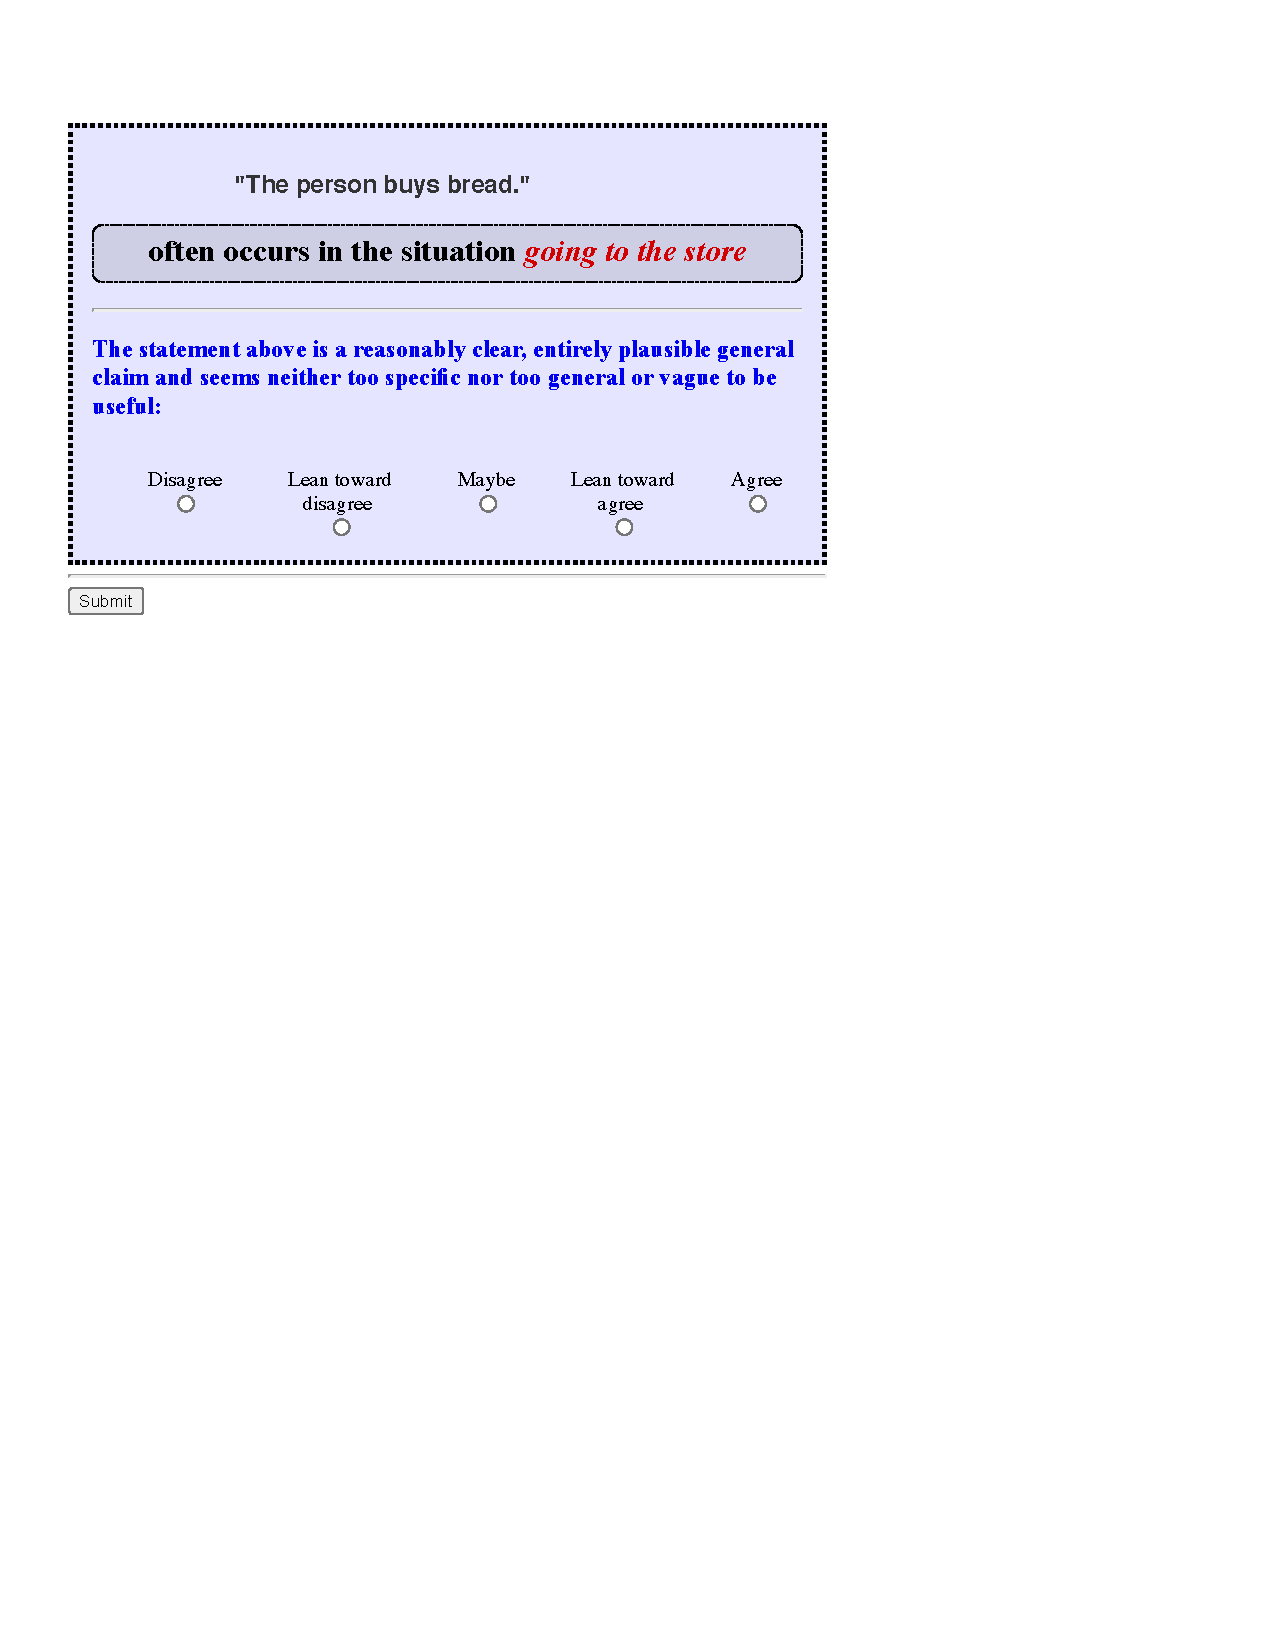
\includegraphics[width=0.5\textwidth]{CH5_eval/gpteval}
    \caption{An example of a form presented to a schema quality evaluator for a \textit{step} formula that has been rendered, using GPT-2, into natural English. This corresponds to the \textit{tabular} version shown in Figure~\ref{fig:step_eval_eg}.}
    \label{fig:gpt_step_eval_eg}
\end{figure}

\section{Inference Evaluation}
\label{sec:inf_eval}

\begin{figure}
    \centering
    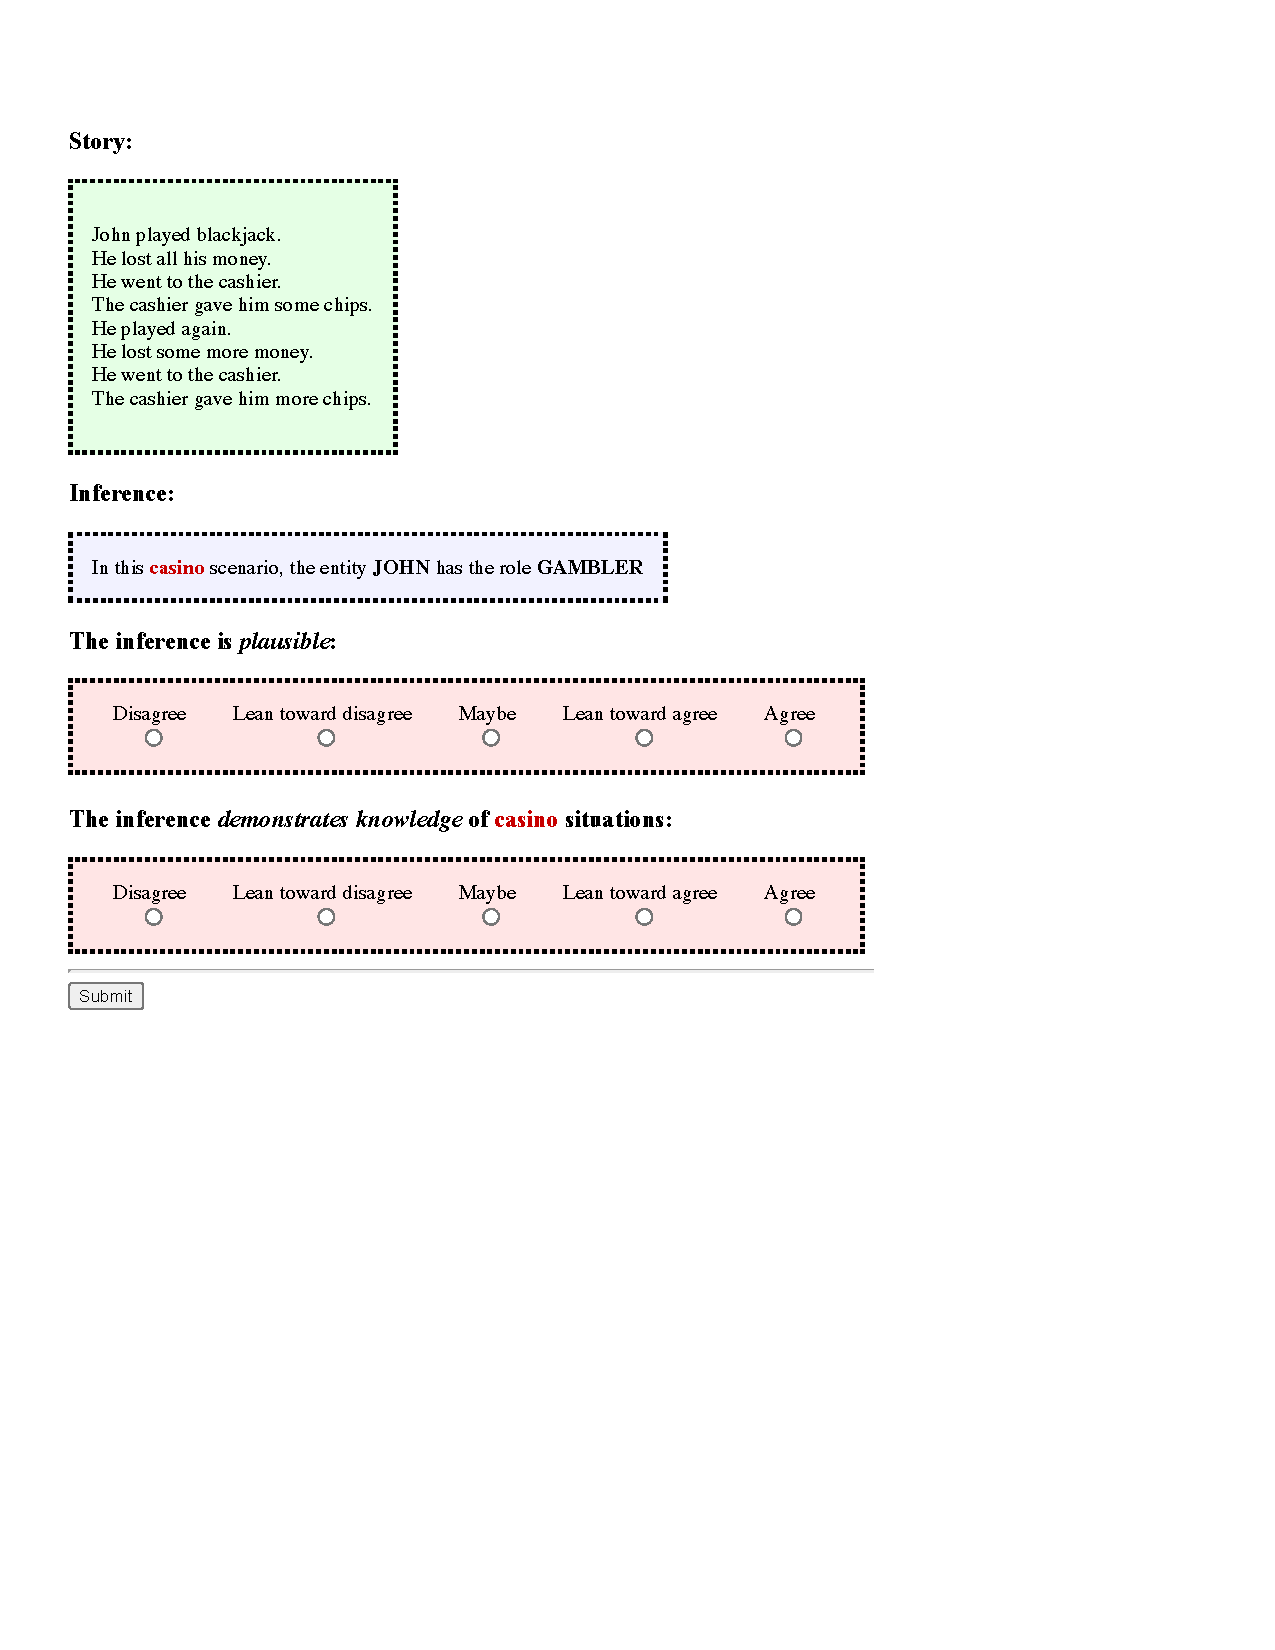
\includegraphics[width=\textwidth]{CH5_eval/role_inf.pdf}
    \caption{An example of a form presented to a schema quality evaluator for a \textit{goal} formula.}
    \label{fig:role_inf_eval}
\end{figure}

\begin{figure}
    \centering
    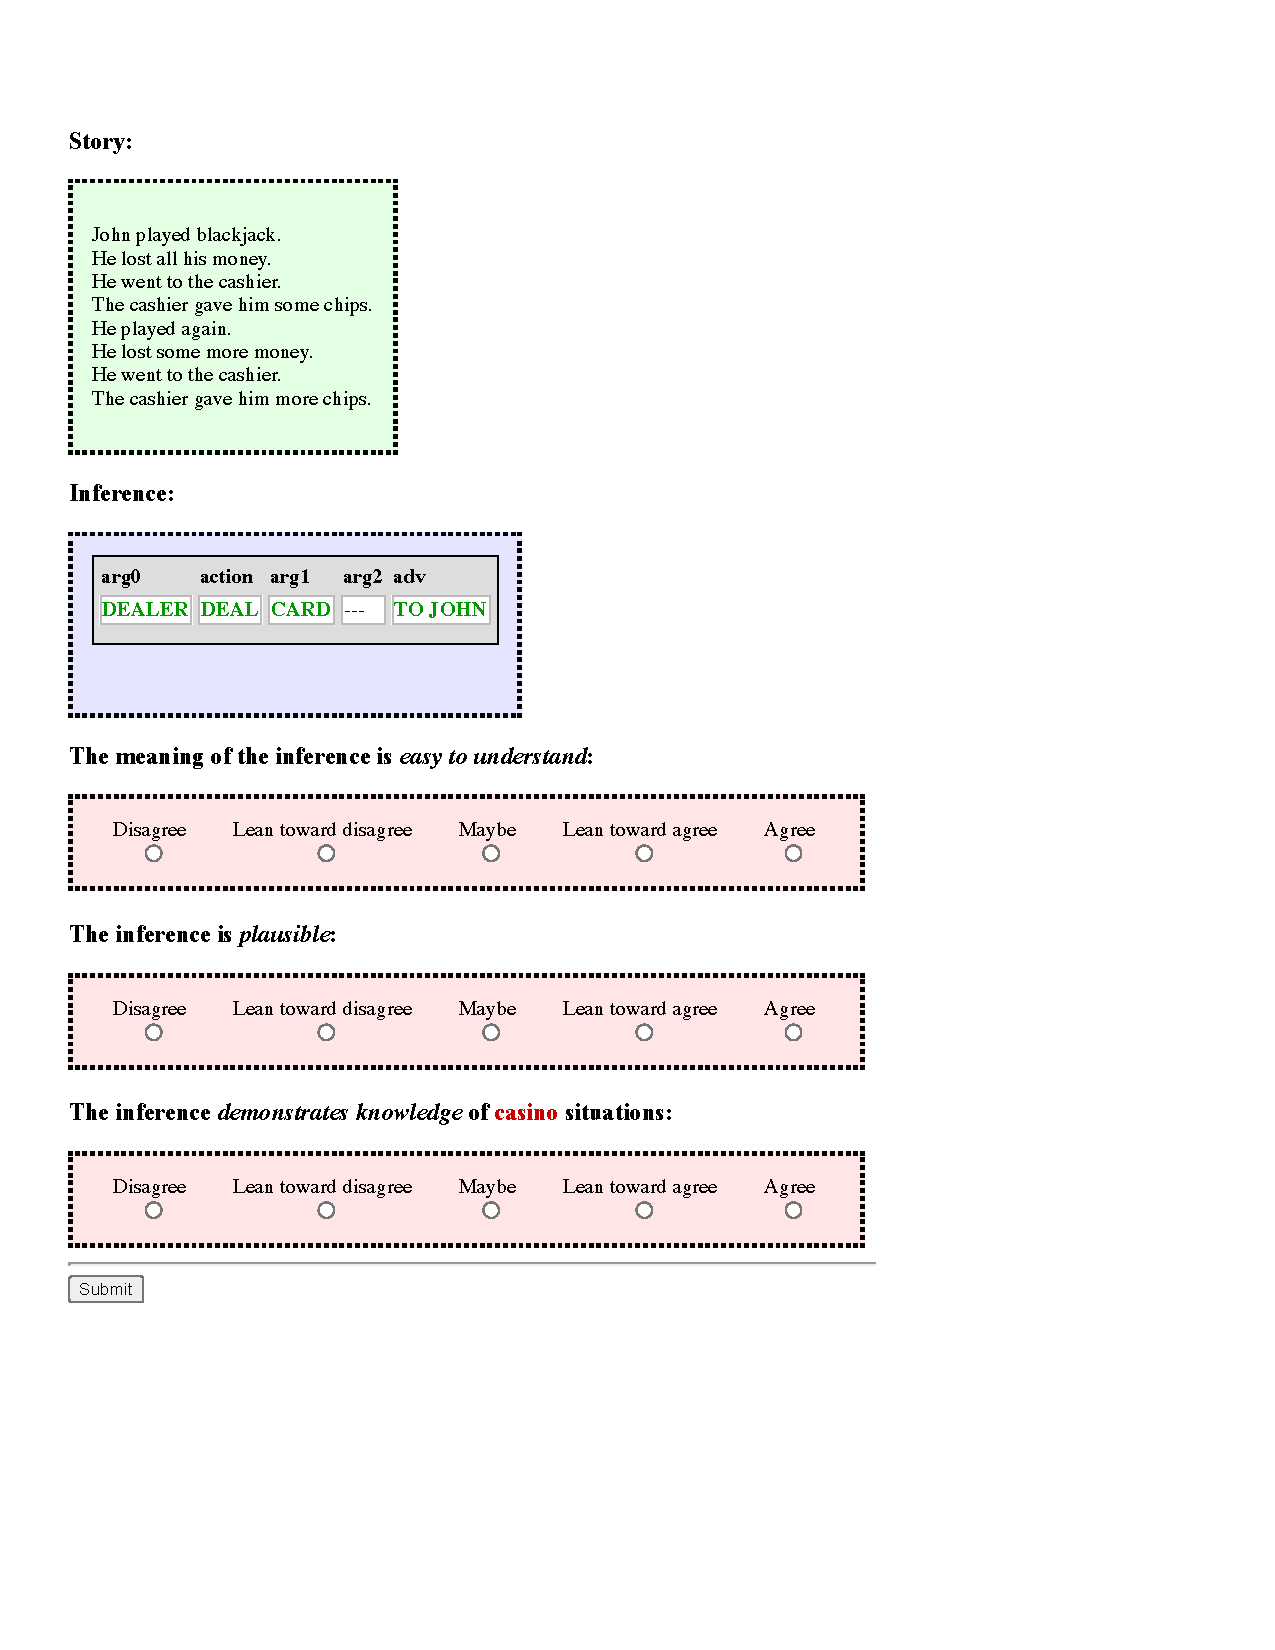
\includegraphics[width=0.75\textwidth]{CH5_eval/step_inf.pdf}
    \caption{An example of a form presented to a schema quality evaluator for a \textit{goal} formula.}
    \label{fig:step_inf_eval}
\end{figure}